\documentclass[12pt, titlepage]{article}

\usepackage{fullpage}
\usepackage[round]{natbib}
\usepackage{multirow}
\usepackage{booktabs}
\usepackage{tabularx}
\usepackage{graphicx}
\usepackage{float}
\usepackage{hyperref}
\usepackage{enumitem}
\hypersetup{
    colorlinks,
    citecolor=blue,
    filecolor=black,
    linkcolor=red,
    urlcolor=blue
}

%% Comments

\usepackage{color}

\newif\ifcomments\commentstrue %displays comments
%\newif\ifcomments\commentsfalse %so that comments do not display

\ifcomments
\newcommand{\authornote}[3]{\textcolor{#1}{[#3 ---#2]}}
\newcommand{\todo}[1]{\textcolor{red}{[TODO: #1]}}
\else
\newcommand{\authornote}[3]{}
\newcommand{\todo}[1]{}
\fi

\newcommand{\wss}[1]{\authornote{blue}{SS}{#1}} 
\newcommand{\plt}[1]{\authornote{magenta}{TPLT}{#1}} %For explanation of the template
\newcommand{\an}[1]{\authornote{cyan}{Author}{#1}}

%% Common Parts

\newcommand{\progname}{ProgName} % PUT YOUR PROGRAM NAME HERE
\newcommand{\authname}{Team \#, Team Name
\\ Student 1 name
\\ Student 2 name
\\ Student 3 name
\\ Student 4 name} % AUTHOR NAMES                  

\usepackage{hyperref}
    \hypersetup{colorlinks=true, linkcolor=blue, citecolor=blue, filecolor=blue,
                urlcolor=blue, unicode=false}
    \urlstyle{same}
                                


\newcounter{acnum}
\newcommand{\actheacnum}{AC\theacnum}
\newcommand{\acref}[1]{AC\ref{#1}}

\newcounter{ucnum}
\newcommand{\uctheucnum}{UC\theucnum}
\newcommand{\uref}[1]{UC\ref{#1}}

\newcounter{mnum}
\newcommand{\mthemnum}{M\themnum}
\newcommand{\mref}[1]{M\ref{#1}}

\begin{document}

\title{Module Guide for \progname{}} 
\author{\authname}
\date{\today}

\maketitle

\pagenumbering{roman}

\section{Revision History}

\begin{table}[hp]
		\centering
		\begin{tabularx}{\textwidth}{lllX}
			\toprule
			\textbf{Revision Version} & \textbf{Date} & \textbf{Developer(s)} & \textbf{Change}\\
			\midrule
			0 & January 17, 2024 & Sam, Sophie, Jonathan, Daniel & First draft of Document\\
			\bottomrule
		\end{tabularx}
	\end{table}



\newpage

\section{Reference Material}

This section records information for easy reference.

\subsection{Abbreviations and Acronyms}

\renewcommand{\arraystretch}{1.2}
\begin{tabular}{l l} 
  \toprule		
  \textbf{symbol} & \textbf{description}\\
  \midrule 
  AC & Anticipated Change\\
  DAG & Directed Acyclic Graph \\
  M & Module \\
  MG & Module Guide \\
  OS & Operating System \\
  R & Requirement\\
  SC & Scientific Computing \\
  SRS & Software Requirements Specification\\
  \progname & Explanation of program name\\
  UC & Unlikely Change \\
  \bottomrule
\end{tabular}\\

\newpage

\tableofcontents

\listoftables

\listoffigures

\newpage

\pagenumbering{arabic}

\section{Introduction}

Breaking down a system into modules is a widely accepted strategy in software development. A module serves as a task assignment for a programmer or programming team. Our approach advocates decomposition based on the principle of information hiding. This principle aligns with designing for change, as the concealed "secrets" within each module anticipate potential future modifications. Designing for change is particularly valuable in SC, where alterations are frequent, especially during the initial development phase as the solution space is explored.

Our design follows the rules, as follows:
\begin{itemize}
\item System details that are likely to change independently should be the
  secrets of separate modules.
\item Each data structure is implemented in only one module.
\item Any other program that requires information stored in a module's data
  structures must obtain it by calling access programs belonging to that module.
\end{itemize}

After completing the first stage of the design, the Software Requirements
Specification (SRS), the Module Guide (MG) is developed [\textit{ParnasEtAl1984}]. The MG
specifies the modular structure of the system and is intended to allow both
designers and maintainers to easily identify the parts of the software.  The
potential readers of this document are as follows:

\begin{itemize}
\item New project members: This document can be a guide for a new project member
  to easily understand the overall structure and quickly find the
  relevant modules they are searching for.
\item Maintainers: The hierarchical structure of the module guide improves the
  maintainers' understanding when they need to make changes to the system. It is
  important for a maintainer to update the relevant sections of the document
  after changes have been made.
\item Designers: Once the module guide has been written, it can be used to
  check for consistency, feasibility, and flexibility. Designers can verify the
  system in various ways, such as consistency among modules, feasibility of the
  decomposition, and flexibility of the design.
\end{itemize}

The rest of the document is organized as follows. Section
\ref{SecChange} lists the anticipated and unlikely changes of the software
requirements. Section \ref{SecMH} summarizes the module decomposition that
was constructed according to the likely changes. Section \ref{SecConnection}
specifies the connections between the software requirements and the
modules. Section \ref{SecMD} gives a detailed description of the
modules. Section \ref{SecTM} includes two traceability matrices. One checks
the completeness of the design against the requirements provided in the SRS. The
other shows the relation between anticipated changes and the modules. Section
\ref{SecUse} describes the use relation between modules.

\section{Anticipated and Unlikely Changes} \label{SecChange}

This section lists possible changes to the system. According to the likeliness
of the change, the possible changes are classified into two
categories. Section \ref{SecAchange} lists anticipated changes, and Section \ref{SecUchange} lists unlikely changes.

\subsection{Anticipated Changes} \label{SecAchange}

Anticipated changes are the source of the information that is to be hidden
inside the modules. Ideally, changing one of the anticipated changes will only
require changing the one module that hides the associated decision. The approach
adapted here is called design for
change.

\begin{description}
\item[\refstepcounter{acnum} \actheacnum \label{acInput}:] The format of the
  initial input data.
\item[\refstepcounter{acnum} \actheacnum \label{acExercise}:] The exercises included in the exercise list.
\item[\refstepcounter{acnum} \actheacnum \label{acProfile}:] The parameters a user can edit for their profile.
\item[\refstepcounter{acnum} \actheacnum \label{acFeedback}:] The feedback form prompts and interaction.
\item[\refstepcounter{acnum} \actheacnum \label{acAlgorithm}:] Algorithm improvement for workout generation.
\end{description}

\subsection{Unlikely Changes} \label{SecUchange}

The module design should be as general as possible. However, a general system is
more complex. Sometimes this complexity is not necessary. Fixing some design
decisions at the system architecture stage can simplify the software design. If
these decision should later need to be changed, then many parts of the design
will potentially need to be modified. Hence, it is not intended that these
decisions will be changed.

\begin{description}
\item[\refstepcounter{ucnum} \uctheucnum \label{ucIO}:] Input/Output devices
  (Input: File and/or Keyboard, Output: File, Memory, and/or Screen).
\item [\refstepcounter{ucnum} \uctheucnum \label{ucEncryption}:] The encryption scheme of data.
\end{description}

\section{Module Hierarchy} \label{SecMH}

This section provides an overview of the module design. Modules are summarized
in a hierarchy decomposed by secrets in Table \ref{TblMH}. The modules listed
below, which are leaves in the hierarchy tree, are the modules that will
actually be implemented.

\begin{description}
\item [\refstepcounter{mnum} \mthemnum \label{mUP}:] User Profile Management Module
\item [\refstepcounter{mnum} \mthemnum \label{mWG}:] Workout Generation Module
\item [\refstepcounter{mnum} \mthemnum \label{mDM}:] Data Management Module
\item [\refstepcounter{mnum} \mthemnum \label{mUI}:] User Interaction Module
\item [\refstepcounter{mnum} \mthemnum \label{mRF}:] Reporting and Feedback Module
\item [\refstepcounter{mnum} \mthemnum \label{mCI}:] ChatBot Integration Module
\item [\refstepcounter{mnum} \mthemnum \label{mAS}:] Algorithm Selection Module
\item [\refstepcounter{mnum} \mthemnum \label{mIF}:] Input Format Module
\end{description}

\begin{table}[h!]
\centering
\begin{tabular}{p{0.3\textwidth} p{0.6\textwidth}}
\toprule
\textbf{Level 1} & \textbf{Level 2}\\
\midrule


\multirow{7}{0.3\textwidth}{Behaviour-Hiding} & User Profile Management Module\\
& Workout Generation Module\\
& Data Management Module\\
& User Interaction Module\\ 
& Reporting and Feedback Module\\
& Chatbot System Module\\
\midrule

\multirow{3}{0.3\textwidth}{Software Decision} & Algorithm Selection Module\\
& Input Format Module\\
\bottomrule

\end{tabular}
\caption{Module Hierarchy}
\label{TblMH}
\end{table}


\section{Connection Between Requirements and Design} \label{SecConnection}

The design of the system is intended to satisfy the requirements developed in
the SRS. In this stage, the system is decomposed into modules. The connection
between requirements and modules is listed in Table~\ref{TblRT}.

\setlength{\parindent}{0cm}
\section{Module Decomposition} \label{SecMD}

The SweatSmart application is composed of several distinct modules, each responsible for a separate concern within the system. This modular approach ensures that each part of the application can be developed, tested, and maintained in isolation, promoting a scalable and robust software architecture. \\

The following sections detail the specific responsibilities and design of each module, providing insight into their individual functions as well as their interactions with other parts of the system. The decomposition is designed to encapsulate core functionalities and to define clear boundaries and interfaces for interaction, facilitating a plug-and-play architecture that can evolve as new features and requirements emerge.\\

Each module is described with an emphasis on its ``secret'' – the design and knowledge it hides from other modules, its interface – the access points for other parts of the system to interact with it, and its interaction with other modules, which delineates how it cooperates within the system to deliver cohesive functionality. \\

The primary modules identified for the SweatSmart application are as follows:

\begin{itemize}
    \item User Profile Module
    \item Workout Generation Module
    \item Data Management Module
    \item User Interaction Module
    \item Reporting and Feedback Module
    \item Algorithm Selection Module
    \item Input Format Module
\end{itemize}

In subsequent sections, we will delve into the particulars of each module, starting with the User Profile Module.

\subsection{Behaviour-Hiding Module}

\subsubsection{User Profile Management Module (M1)}

The User Profile Management Module is central to the personalization features of the SweatSmart application. Its primary responsibility is to manage user-specific data, which includes account creation, user authentication, and the storage and retrieval of personal fitness profiles.

\begin{description}[leftmargin=0pt]
\item[Secrets:] 
The module encapsulates the logic for user data validation, ensuring that data integrity is maintained and personal information is stored securely. It also handles the encryption and decryption of sensitive information to protect user privacy. Additionally, this module will include logic to provide data in the format expected by the Algorithm Selection Module for personalized workout algorithms.
\end{description}

\begin{description}[leftmargin=0pt] % Add style=nextline to ensure the title and 
\item[Services:] 
\end{description}
\begin{itemize}[leftmargin=*]
\item Account creation and management.
\item User login and authentication processes.
\item Personal information updates and management.
\item Privacy settings and account security features.
\item Services for formatting user data as per the standards defined in the Input Format Module.
\end{itemize}

\begin{description}[leftmargin=0pt]
\item[Interfaces:] 
\end{description}
\begin{itemize}[leftmargin=*]
\item An API endpoint for account creation and modification.
\item Authentication services that integrate with third-party identity providers.
\end{itemize}

By maintaining a clear separation of concerns, the User Profile Management Module ensures that user-related features are modular, scalable, and independent, enabling effective and secure management of user-specific data within the broader SweatSmart system. This module's design will provide potential for future enhancements such as integration with social media platforms for enriched user profiles and community engagement.


\subsubsection{Workout Generation Module (M2)}

The Workout Generation Module is the central aspect of the SweatSmart application, responsible for curating personalized workout plans tailored to the individual user's fitness goals, preferences, and progress.

\begin{description}[leftmargin=0pt]
\item[Secrets:] 
The module is designed to hold evidence-based algorithms that consider a range of variables such as the user's exercise history, current fitness level, performance metrics, and personal targets. It ensures that workouts are challenging and effective, promoting consistent user progress. It will refer to the Algorithm Selection Module for choosing the appropriate workout generation algorithm.
\end{description}

\begin{description}[leftmargin=0pt]
\item[Services:] 
\end{description}
\begin{itemize}[leftmargin=*]
\item Creation of personalized workout routines.
\item Adaptation of workouts in response to user feedback.
\item Dynamic adjustment to plans based on user feedback and workout results.
\item Integration of rest and active days to optimize recovery and growth.
\item Receives pre-validated and formatted data from the Input Format Module.
\end{itemize}

\begin{description}[leftmargin=0pt]
\item[Interfaces:] 
\end{description}
\begin{itemize}[leftmargin=*]
\item API endpoints for initiating workout generation and retrieving the latest plans.
\item Interfaces to receive user data updates from the User Profile Management Module.
\item Output methods to deliver the workout plan to the User Interaction Module.
\end{itemize}

Interaction with Other Modules: The Workout Generation Module interacts extensively with the User Profile Management Module to obtain necessary user data. The module also feeds data to the Reporting and Feedback Module to inform users of their progress and areas for improvement. Its algorithms can be updated or enhanced based on patterns observed from the Data Management Module, ensuring the workouts remain effective as fitness sciences evolve.
\\

By maintaining this modular approach, the Workout Generation Module can be independently updated or replaced if new fitness planning methodologies are adopted, without the need to overhaul the entire system. This ensures that SweatSmart can remain at the cutting edge of fitness evidence, providing users with effective, science-backed workout regimens.

\subsubsection{Data Management Module (M3)}

The Data Management Module in SweatSmart is integral for handling all data storage, retrieval, and management operations. It ensures efficient and secure handling of user data, workout logs, and application metrics.

\begin{description}[leftmargin=0pt]
\item[Secrets:] 
The module encapsulates the database schema design, data access layers, and the data querying logic. It is responsible for ensuring data integrity, consistency, and optimizing data retrieval and storage operations. This module also interfaces with the Input Format Module to ensure all data stored and retrieved is correctly formatted.
\end{description}

\begin{description}[leftmargin=0pt]
\item[Services:] 
\end{description}
\begin{itemize}[leftmargin=*]
\item Secure storage of user profiles, workout histories, and preferences.
\item Efficient retrieval of data for real-time application use.
\item Management of data backups and restoration processes.
\item Implementation of data privacy and protection mechanisms.
\item Formats data according to the rules of the Input Format Module before storage.
\end{itemize}

\begin{description}[leftmargin=0pt]
\item[Interfaces:] 
\end{description}
\begin{itemize}[leftmargin=*]
\item APIs for data CRUD (Create, Read, Update, Delete) operations.
\item Interfaces to interact with the User Profile Management and Workout Generation Modules for data exchange.
\item Data export functions for reporting and analysis purposes.
\end{itemize}

Interaction with Other Modules: The Data Management Module serves as the backbone for the User Profile Management and Workout Generation Modules, providing them with necessary data. It also interacts with the Reporting and Feedback Module to supply data for generating user reports and analytics.
\\

By centralizing data management, SweatSmart ensures that all modules have consistent and reliable access to the necessary data, enhancing the application's overall performance and user experience.

\subsubsection{User Interaction Module (M4)}

The User Interaction Module is a pivotal component of SweatSmart, focusing on the user interface (UI) and user experience (UX) aspects of the application. It facilitates the interaction between the user and the software's functionalities.

\begin{description}[leftmargin=0pt]
\item[Secrets:] 
This module contains the design elements, layout configurations, and interaction logic that define how users interact with the application. It ensures a seamless, intuitive, and engaging user experience. It also contains the logic to handle formatting feedback data from the Input Format Module to be sent to other modules.
\end{description}

\begin{description}[leftmargin=0pt]
\item[Services:] 
\end{description}
\begin{itemize}[leftmargin=*]
\item Rendering of the user interface, including screens for profile management, workout plans, and feedback.
\item Handling user inputs and translating them into actions within the application.
\item Displaying personalized content and workout suggestions.
\item Alerting users when input data does not meet formatting requirements.
\end{itemize}

\begin{description}[leftmargin=0pt]
\item[Interfaces:] 
\end{description}
\begin{itemize}[leftmargin=*]
\item Front-end frameworks and libraries for UI rendering.
\item API endpoints for sending user inputs to backend modules and receiving data.
\item Integration with Workout Generation Module for real-time data display.
\end{itemize}

Interaction with Other Modules: The User Interaction Module is closely linked with almost all other modules. It receives data from the Data Management Module for display and sends user inputs back for processing. It also works in conjunction with the Workout Generation Module to present tailored workout plans to enhance user engagement.
\\

By focusing on a user-centric design, this module plays a crucial role in ensuring that SweatSmart is not only functional but also enjoyable and easy to use.

\subsubsection{Reporting and Feedback Module (M5)}

The Reporting and Feedback Module is a key component of SweatSmart, focusing on the collection, analysis, and presentation of user feedback and workout data. This module is instrumental in understanding user satisfaction and system performance.

\begin{description}[leftmargin=0pt]
\item[Secrets:]
The module houses the mechanisms for gathering user feedback, analyzing workout data, and generating reports. It ensures confidentiality and accuracy in feedback processing and report generation. It includes the decision-making logic provided by the Algorithm Selection Module for generating insights based on user feedback.
\end{description}

\begin{description}[leftmargin=0pt]
\item[Services:]
\end{description}
\begin{itemize}[leftmargin=*]
\item Collection and storage of user feedback from various points within the app.
\item Analysis of workout data to generate performance reports.
\item Generation of insights based on user activity and feedback.
\item Formats feedback data from users according to standards set by the Input Format Module.
\end{itemize}

\begin{description}[leftmargin=0pt]
\item[Interfaces:]
\end{description}
\begin{itemize}[leftmargin=*]
\item Feedback collection interfaces within the app.
\item Reporting APIs to deliver analyzed data and insights to users and administrators.
\item Data exchange interfaces with the Data Management Module for accessing user data.
\end{itemize}

Interaction with Other Modules: The Reporting and Feedback Module interacts with the User Profile Management Module to tailor feedback requests based on user profiles. It also collaborates with the Workout Generation Module by providing insights that can be used to refine the workout algorithms. Interaction with the Data Management Module is crucial for accessing and storing the necessary data for analysis.
\\

This module plays a vital role in driving improvements across the SweatSmart platform by translating user feedback and workout data into actionable insights.

\subsubsection{ChatBot Integration Module (M6)}

The ChatBot Integration Module serves as the intermediary between the SweatSmart application and OpenAI's Chat GPT API, enabling advanced conversational capabilities and interactive user support within the application.

\begin{description}[leftmargin=0pt]
\item[Secrets:] 
This module encapsulates the logic for interacting with the Chat GPT API, including constructing the HTTP requests, managing authentication, handling the conversation state, and parsing the responses. It abstracts the complexities of network communication, JSON serialization, and API key management, ensuring these implementation details are not exposed to the other parts of the system.
\end{description}

\begin{description}[leftmargin=0pt]
\item[Services:]
\end{description}
\begin{itemize}[leftmargin=*]
\item Authenticate and communicate with the OpenAI Chat GPT API.
\item Send user messages and system context to the API and receive responses.
\item Serialize and deserialize chat messages to and from JSON format.
\item Manage API keys securely, retrieving them from Azure Key Vault when not available in the environment variables.
\end{itemize}

\begin{description}[leftmargin=0pt]
\item[Interfaces:]
\end{description}
\begin{itemize}[leftmargin=*]
\item RESTful API endpoints to receive chat messages from the client and send responses back.
\item Authentication interface to secure chat endpoints.
\end{itemize}

\textbf{Interaction with Other Modules:} 
The ChatBot Module interacts with the User Profile Management Module to retrieve user preferences and context for personalized interactions. It also connects with the Data Management Module to store and retrieve conversation histories.

By integrating with OpenAI's Chat GPT API, the ChatBot Module provides a robust solution for real-time user interaction, leveraging the capabilities of AI to deliver personalized and intelligent support within the SweatSmart application.



\subsection{Software Decision Module}

\subsubsection{Algorithm Selection Module (M7)}

The Algorithm Selection Module is a crucial software decision-making component of SweatSmart, responsible for determining the most effective algorithms for workout generation and analytics based on real-time user data.

\begin{description}[leftmargin=0pt]
\item[Secrets:]
The module comprises advanced selection logic to choose the optimal algorithm for each user, considering factors like past performance, current fitness levels, and user preferences. This module also includes proprietary methods for evaluating and comparing the effectiveness of different algorithms.
\end{description}

\begin{description}[leftmargin=0pt]
\item[Services:]
\end{description}
\begin{itemize}[leftmargin=*]
\item Dynamic selection of workout and analytics algorithms based on user data.
\item Periodic evaluation of algorithm effectiveness and adaptation as necessary.
\item Provision of a selection interface for other modules to request algorithm services.
\end{itemize}

\begin{description}[leftmargin=0pt]
\item[Interfaces:]
\end{description}
\begin{itemize}[leftmargin=*]
\item Algorithm selection interface used by the Workout Generation and Predictive Analytics Modules.
\item Interface for receiving user data and preferences from the User Profile Management Module.
\end{itemize}

Interaction with Other Modules: The Algorithm Selection Module directly impacts the functionality of the Workout Generation Module by supplying it with the appropriate algorithm for creating personalized workout plans. It also interacts with the Reporting and Feedback Module to use insights from user feedback for algorithm refinement.
\\

By effectively selecting and managing the algorithms used across the application, the Algorithm Selection Module ensures that SweatSmart adapts to the unique and changing needs of each user, providing a highly personalized fitness experience.

\subsubsection{Input Format Module (M8)}

The Input Format Module is an integral part of SweatSmart, ensuring all user and system data is correctly formatted and validated before being processed by the application's various functional components.

\begin{description}[leftmargin=0pt]
\item[Secrets:]
This module harbors the logic for data validation rules, format specifications, and sanitization procedures. It acts as the first line of defense against data inconsistencies and errors that could compromise system functionality.
\end{description}

\begin{description}[leftmargin=0pt]
\item[Services:]
\end{description}
\begin{itemize}[leftmargin=*]
\item Validation and formatting of incoming data from user inputs and external sources.
\item Sanitization of data to remove or correct any inaccuracies or inconsistencies.
\item Provision of formatting rules and validation interfaces for other system modules.
\end{itemize}

\begin{description}[leftmargin=0pt]
\item[Interfaces:]
\end{description}
\begin{itemize}[leftmargin=*]
\item Data validation and formatting interface utilized by the User Interaction Module.
\item Sanitization interface for cleaning data received from External Integration Module.
\end{itemize}

Interaction with Other Modules: The Input Format Module serves all other modules by ensuring the data they receive is in the correct format and meets the system's data quality standards. It plays a critical role in the interaction between the User Interaction Module and the core system components, such as the Workout Generation and Predictive Analytics Modules, by providing them with clean and standardized data.
\\

By maintaining the integrity and consistency of the data throughout SweatSmart, the Input Format Module supports robust system operations and a seamless user experience.


%\setlength{\parindent}{default}

\section{Traceability Matrix} \label{SecTM}

This section shows two traceability matrices: between the modules and the
requirements and between the modules and the anticipated changes.

% the table should use mref, the requirements should be named, use something
% like fref
\begin{table}[H]
\centering
\begin{tabular}{p{0.2\textwidth} p{0.6\textwidth}}
\toprule
\textbf{Requirement} & \textbf{Modules}\\
\midrule
UA1 & \mref{mUP}, \mref{mDM}, \mref{mUI}, \mref{mIF}\\
UA2 & \mref{mUP}, \mref{mDM}, \mref{mUI}, \mref{mAS}\\
UA3 & \mref{mUP}, \mref{mDM}, \mref{mUI}, \mref{mAS}\\
UA4 & \mref{mUP}, \mref{mUI}, \mref{mAS}\\
UA5 & \mref{mUP}, \mref{mUI}, \mref{mAS}\\
AI1 & \mref{mUP}, \mref{mWG}, \mref{mDM}, \mref{mUI}, \mref{mAS}\\
AI2 & \mref{mWG}, \mref{mDM}, \mref{mAS}\\
AI3 & \mref{mWG}, \mref{mDM}, \mref{mRF}, \mref{mAS}\\
AI4 & \mref{mDM}, \mref{mUI}, \mref{mCI}\\
AI5 & \mref{mDM}, \mref{mUI}, \mref{mRF}, \mref{mAS}\\
UC1 & \mref{mUP}, \mref{mWG}, \mref{mDM}, \mref{mUI}\\
UC2 & \mref{mUI}, \mref{mRF}\\
UC3 & \mref{mUP}, \mref{mDM}, \mref{mUI}\\
UC4 & \mref{mDM}\\
WH1 & \mref{mUP}, \mref{mDM}\\
WH2 & \mref{mDM}, \mref{mRF}\\
DB1 & \mref{mUP}, \mref{mWG}, \mref{mDM}, \mref{mUI}, \mref{mRF}\\
AF1 & \mref{mUI}, \mref{mAS}\\
AF2 & \mref{mDM}, \mref{mUI}\\
AF3 & \mref{mUP}, \mref{mWG}, \mref{mDM}, \mref{mUI} \\
AF4 & \mref{mUP}, \mref{mDM} \\
AF5 & \mref{mUP}, \mref{mDM}, \mref{mUI}\\
\bottomrule
\end{tabular}
\caption{Trace Between Requirements and Modules}
\label{TblRT}
\end{table}

\begin{table}[H]
\centering
\begin{tabular}{p{0.2\textwidth} p{0.6\textwidth}}
\toprule
\textbf{AC} & \textbf{Modules}\\
\midrule
\acref{acInput} & \mref{mIF}\\
\acref{acExercise} & \mref{mDM}\\
\acref{acProfile} & \mref{mUP}\\
\acref{acFeedback} & \mref{mRF}\\
\acref{acAlgorithm} & \mref{mAS}\\
\bottomrule
\end{tabular}
\caption{Trace Between Anticipated Changes and Modules}
\label{TblACT}
\end{table}

\section{Use Hierarchy Between Modules} \label{SecUse}

In this section, the uses hierarchy between modules is
provided. \textit{Parnas1978} said of two programs A and B that A {\em uses} B if
correct execution of B may be necessary for A to complete the task described in
its specification. That is, A {\em uses} B if there exist situations in which
the correct functioning of A depends upon the availability of a correct
implementation of B.  Figure \ref{FigUH} illustrates the use relation between
the modules. It can be seen that the graph is a directed acyclic graph
(DAG). Each level of the hierarchy offers a testable and usable subset of the
system, and modules in the higher level of the hierarchy are essentially simpler
because they use modules from the lower levels.

\begin{figure}[H]
\centering
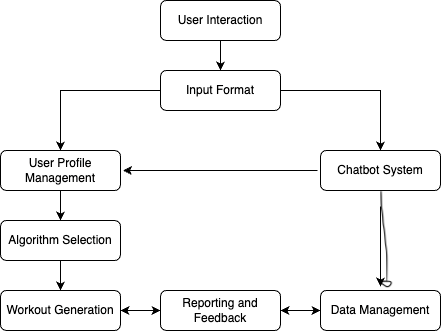
\includegraphics[width=0.7\textwidth]{docs/design/SoftArchitecture/UseHierarchyModules.png}
\caption{Use hierarchy among modules}
\label{FigUH}
\end{figure}

%\section*{References}

%\bibliographystyle {plainnat}
%\bibliography{../../../refs/References}

\newpage{}

\section{Timeline}
\begin{table}[H]
\centering
\begin{tabular}{lll}
\toprule
\textbf{Module} & \textbf{Developers} & \textbf{Deadline}\\
\midrule
M1 & Daniel, Jonathan & Feb 2, 2024\\
M2 & Sam, Sophie & Jan 27, 2024\\
M3 & Daniel, Jonathan, Sam, Sophie & Feb 2, 2024\\
M4 & Daniel, Jonathan, Sam, Sophie & Feb 2, 2024\\
M5 & Daniel, Jonathan, Sam, Sophie & Feb 2, 2024\\
M6 & Daniel, Sophie & Jan 25, 2024\\
M7 & Sam, Sophie & Jan 27, 2024\\
M8 & Daniel, Jonathan & Jan 31, 2024\\
\bottomrule
\end{tabular}
\caption{Timeline for Revision 0 Demo}
\label{TblT}
\end{table}

\end{document}
